\documentclass[
    parskip=half, 
    twoside=false,
    twocolumn=true,
    fontsize=11pt,
]{scrarticle}
\usepackage{xcolor}
\definecolor{seeblau}{HTML}{00A9E0}
\definecolor{seegrau}{HTML}{9AA0A7}

\definecolor{seeblau1}{HTML}{CCEEF9}
\definecolor{seeblau2}{HTML}{A6E1F4}
\definecolor{seeblau3}{HTML}{59C7EB}
\definecolor{seeblau4}{HTML}{00A9E0}
\definecolor{seeblau5}{HTML}{008ECE}


\usepackage{graphicx}
\usepackage{amsmath}
\usepackage{subcaption}
\usepackage{wrapfig}
\usepackage[english]{babel}
\usepackage{blindtext}
\usepackage{microtype}
\usepackage{siunitx}
\usepackage[utf8]{inputenc}
\usepackage{csquotes}
\usepackage{nicefrac}
\usepackage[T1]{fontenc}
\usepackage{amsfonts}
\usepackage{amssymb}
\usepackage{tikz}

\usepackage{siunitx}

\usepackage{libertinus, libertinust1math}
\usepackage{roboto}

\setkomafont{disposition}{\normalfont\sffamily}


% not recommended with KOMA-script
% make table of contents sans-serif
% \usepackage{tocloft}
% \renewcommand\cftchappagefont{\normalfont}
% \renewcommand\cftchapfont{\normalfont}
% \renewcommand\cftchappresnum{\bfseries}
% \renewcommand\cftchapaftersnum{}
% \renewcommand{\cftchapfont}{\sffamily}
% \renewcommand{\cftsecfont}{\sffamily}
% \renewcommand{\cftsubsecfont}{\sffamily}
% \renewcommand{\cftchappagefont}{\sffamily}
% \renewcommand{\cftsecpagefont}{\sffamily}
% \renewcommand{\cftsubsecpagefont}{\sffamily}

% caption
\usepackage{caption}
\captionsetup{
	% font={sf},
	labelfont={sf, bf, color=seeblau},
	labelsep=quad,
	labelformat=simple,
}

% links
\usepackage{hyperref}
\hypersetup{
	colorlinks=true,
	linkcolor=seeblau,
	citecolor=seeblau,
	urlcolor=seeblau,
	% hidelinks=true
}

% bibliography
\usepackage[
	style=numeric-comp, % comp = compressed 4,5,6,7 -> 4-7
	sorting=none,		% Sort by appearance
	% autocite = superscript,
	% backref=true,
	hyperref=true,
	url=true,
	maxbibnames=100
]{biblatex}
\DefineBibliographyStrings{english}{%
    backrefpage  = {see p.}, % for single page number
    backrefpages = {see pp.} % for multiple page numbers
}

% remove issue
\AtEveryBibitem{%
  \clearfield{number}
}

\usepackage{float}
% \floatplacement{figure}{h}
% \floatplacement{table}{H}

% loosen float placement rules
\renewcommand{\topfraction}{0.8}
\renewcommand{\bottomfraction}{.8}
\renewcommand{\textfraction}{0.1}
\renewcommand{\floatpagefraction}{.9}
% make floats less likely to be placed on a separate page
\setcounter{totalnumber}{9}
\setcounter{topnumber}{9}
\setcounter{bottomnumber}{9}

% decrease space between floats and text
\setlength{\textfloatsep}{0.5cm}
\setlength{\floatsep}{0.5cm}


\usepackage{adjustbox}

\usepackage{datetime}
\newdateformat{dotdate}{
	\twodigit{\THEDAY}.\twodigit{\THEMONTH}.\THEYEAR
}
\newdateformat{monthyeardate}{%
  \monthname[\THEMONTH] \THEYEAR}


% header and footer
\usepackage[
  markcase=noupper
]{scrlayer-scrpage}% activates pagestyle scrheadings automatically
\clearpairofpagestyles
\setkomafont{pageheadfoot}{\normalfont\sffamily}
\setkomafont{pagenumber}{\normalfont\sffamily}
% \chead*{\color{seegrau} Draft \dotdate\today}
\ofoot*{\pagemark}
\ohead*{\rightmark}


\usepackage{ifthen}
\newcommand{\markieren}[4]{
    \ifthenelse{\equal{#1}{}}{}{\adjustbox{padding=3pt, bgcolor=seeblau1, margin=-1pt}{\strut{\sffamily\robotoMedium{#1}}}\\}
    \ifthenelse{\equal{#2}{}}{}{\adjustbox{padding=3pt, bgcolor=seeblau2, margin=-1pt}{\strut{\sffamily\robotoMedium{#2}}}\\}
	\ifthenelse{\equal{#3}{}}{}{\adjustbox{padding=3pt, bgcolor=seeblau3, margin=-1pt}{\strut{\sffamily\robotoMedium{#3}}}\\}
	\ifthenelse{\equal{#4}{}}{}{\adjustbox{padding=3pt, bgcolor=seeblau4, margin=-1pt}{\strut{\sffamily\robotoMedium{#4}}}}
}

\addbibresource{literature.bib}

\begin{document}

\title{title}
\subtitle{subtitle}
\author{Aurel Müller-Schoenau, Leon Oleschko}
\date{\dotdate\today}


% make a custom title page
\begin{titlepage}
    \sffamily
    \vspace*{3cm}
    {
        \fontsize{32}{32}
        \markieren{}{}{}{Motencarlo}
    }
    \vspace{.25cm}\\
    {
        \Large
        Aurel Müller-Schoenau, Leon Oleschko\\
        Supervised by Philipp Baumgärtel
        \vspace{.05cm}\\
        22.01.2025
        \vspace{.25cm}\\
        \normalsize
        Physikalisches Fortgeschrittenenpraktikum 2\\
        Universität Konstanz
    }
    \vfill
    {
        \normalfont\normalsize
        TODO
    }
    \vfill
    \begin{flushright}
        Available at \url{www.github.com/leoole100/fp2}.
    \end{flushright}
\end{titlepage}

\section{Introduction}
In physics research we ususally try to rely on very simplified model systems. This lets us investigate dynamics deterministically under controlled conditions to analyse each and every relevant interplay. However, nature is complex and modeling real systems may lead to the question - How do you analyse systems so complex they have a (practically) indefinite amount of degrees of freedom?\\
Statistical physics deals with this issue by making assumptions based on the idea that nature approaches thermodynamic equilibrium. This simplifies the dynamics of a single particle because one may assume the interactions with the rest of the system can be reduced to random interactions following a certain distribution. Computer-based methods making use of random numbers as means for simulation are generally called \textit{Monte-Carlo-Methods}.\\
In this experiment, we simulate the one-dimensional trajectory of a particle inside different energy potential landscapes under the influence of random kicks. Our goal is to confirm the theoretical models derived in statistical mechanics.

\section{Results}
\subsection{Free Particle}
\begin{figure}
\label{fig:pt1_trajectory}
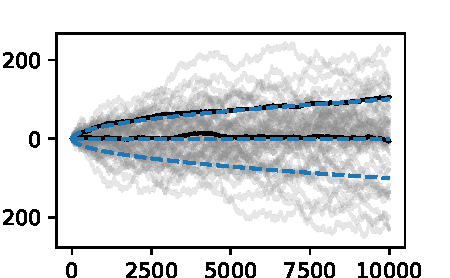
\includegraphics{figures/01 time trace.pdf}
\end{figure}
\begin{figure}
\label{fig:pt1_msd}
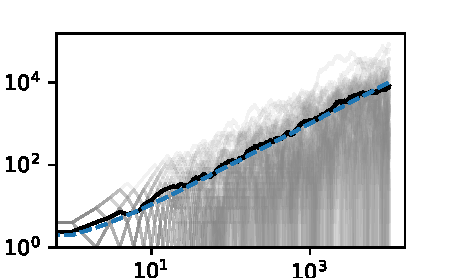
\includegraphics{figures/01 msd.pdf}
\end{figure}

% TODO: Diagramme: Trajektorien, Mean Trajectorien, MSQ mit theoretischer Kurve

In the first part of this experiment, the simple goal was to get a simulation running with nothing more than a freely moving particle in one dimension. The code was written in python and vectorized using NumPy. The trajectory was initialised at position \SI{0}{}. For each timestep, a displacement of $\Delta x_n \in \{\pm \Delta x\}$ was applied in either the positive or negative direction, chosen randomly (at each timestep) with equal probability. This results in Brownian Motion shown in \autoref{fig:pt1_trajectory}. Simulation data was generated for \SI{50} individual trajectories, each one being simulated for a total of $N=\SI{10000}{}$ timesteps. The expected result are freely diffusive dynamics, as shown in the plot. The \textit{Mean Square Displacement} is defined by
\begin{equation}
 MSQ(t_n) = x^2(t_n), \qquad t_n = n \cdot \Delta t
\end{equation}
Since the displacements for different timesteps $t_i\neq t_j$ are uncorrelated, we expect that
\begin{align}
 MSQ(t_n = n \Delta t) &= \left(\sum_{i=1}^n \Delta x_i\right)^2 \\&= 2 \cdot \underbrace{\sum_{i<j\leq n} \Delta x_i \Delta x_j}_{=0} + \sum_{i=1}^n \Delta x_i^2 \\ &= n \cdot \Delta x^2
\end{align}
The MSQ averaged over all \SI{50}{} trajectories is shown in \autoref{fig:pt1_msd} alongside the theoretical prediction.


\subsection{Potential Well}
\begin{figure}
\label{fig:pt2_trajectory}
 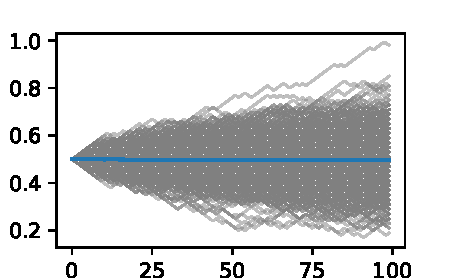
\includegraphics{figures/02 time evolution.pdf}
\end{figure}

Next we looked at a particle trapped inside a potential well with infinitely high walls. This was realised by not allowing displacement across the borders of the well so that the particle was effectively reflected. Inside the well, the potential is flat, resulting in dynamics similar to those of the free particle. \autoref{fig:pt2_trajectory} shows simulation data for \SI{1000}{} trajectories, each with initial position \SI{0.5}{} in the middle of the potential well with borders $0$ and $1$. As one would expect, the mean displacement stays exactly there as the particle cannot escape the potential. The histogram in \autoref{fig:pt2_histogram} shows the average spacial distribution of all trajectories. It is flat, meaning that on average, the particle is able to visit each position of the potential with equal probability. The dip at the starting position is likely a sampling artifact since the histogram grid might not line up with the grid imposed on the particle movement owing to the fact that $\Delta x$ stays constant. In \autoref{fig:pt2_histogram_random} the starting points for the trajectories were randomised to investigate this. A time-resolved version of the same histogram is shown in \autoref{fig:pt2_histogram_time}. Here we can see that for short simulation times, where the particle has not yet been able to interact with the walls, it behaves like the free particle (consider \autoref{fig:pt1_msd}). After evolving for some time, the particle has had a chance to visit each spot, including near the walls and get blocked. With its movement inhibited, it may travel back through the potential, and after sufficiently long simulation time there is no longer any clear structure in the spacial distribution: it approaches a flat line across the entire space available.


\begin{figure}
 \label{fig:pt2_histogram}
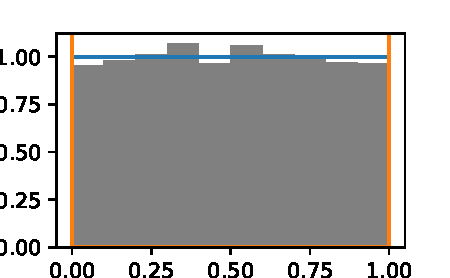
\includegraphics{figures/02 histogram.pdf}
\end{figure}
\begin{figure}
 \label{fig:pt2_histogram_random}
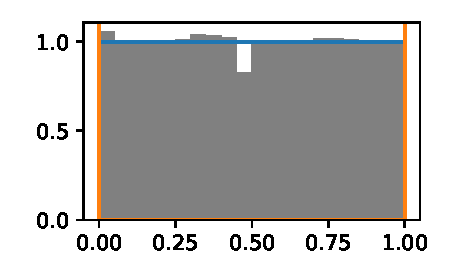
\includegraphics{figures/02 histogram random start.pdf}
\end{figure}
\begin{figure}
 \label{fig:pt2_histogram_time}
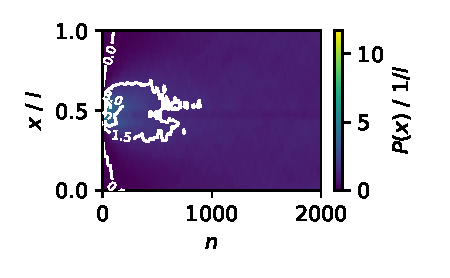
\includegraphics{figures/02 histogram evolution.pdf}
\end{figure}


\subsection{Harmonic Potential}

The harmonic potential appears in many real world cases, and any analytic potential can at least be approximated (locally) quadratically. In our case, the idea is to simulate a particle trapped inside optical tweezers, the resulting potential is nearly harmonic as we learned from one of our previous experiments:
\begin{equation}
 V(x) = \frac{a}{2} x^2
\end{equation}
where $a$ is a constant parameter.\\
Unlike in the previous sections, the particle can now explore areas but only if it gains enough energy. The resulting spacial distribution should be
\begin{equation}
\label{eq:canonical_dist}
 P(x) \propto \exp\left(-\frac{V(x)}{k T}\right)
\end{equation}
where $k T$ is the thermal energy and $V(x)$ is the potential. In order to incorporate this into our simulation, we make use of the \textit{Metropolis Algorithm}: The step size $\Delta x$ stays the same, but the next step is only accepted with a probability of
\begin{equation}
 p(x_i \rightarrow x_{i+1}) = \text{min}\left[1,\exp\left(-\frac{V(x_{i+1})-V(x_i)}{k T}\right)\right]
\end{equation}
meaning that it gets increasingly unlikely that the particle climbs up higher in the potential. Our simulation was run for \SI{2000}{} timesteps and we simulated \SI{500}{} trajectories. All energies were considered relative to the thermal energy, i.e. $kT=1$ and the value of $V(x)$ is to be interpreted in units of $kT$. The results are shown in TODO:FIGURE-HISTOGRAM-HARMONIC in the form of a time-resolved histogram. The spacial distribution follows a normal Distribution as expected, since \autoref{eq:canonical_dist} becomes a Gaussian for $V(x)\propto x^2$.


\subsection{Double Well}

In the final part of the experiment we simulated a particle trapped inside a double-well potential given by
\begin{equation}
 V(x) = a\left(\left(\frac{x}{b}\right)^2-1\right)^2
\end{equation}
which is a fourth order polynomial with minima at $x=\pm b$ and a local maximum inbetween at $x=0$ and $V(x)=a$. Letting the particle evolve freely using the same Metropolis procedure as in the previous section, it delves inside one of the potential wells first, until after some time it manages to climb and surpass the barrier imposed by the local maximum at $x=0$. Our goal was to find out how the time it takes on average to complete one such jump after starting from the bottom of one potential well depends on the height of the barrier $a$. To do this, we simulated many trajectories for many values of $a$. The resulting mean jump times - that is the time between initialisation and the point where the particle reaches the maximum of the barrier - are plotted over the parameter $a$ in TODO:FIGURE-ARRHENIUS. They increase exponentially with $a$ according to TODO:WHATEVER-THE-RELATION-IS

\pagebreak
\section{Conclusion}

The \textit{Monte Carlo Simulation} experiment is a small introduction into physical simulation of systems described by statistical physics. We demonstrated how such simulations are set up for different simulation scenarios. In the first part of the experiment, we simulated a freely moving particle and were able to confirm the viability of the law of free diffusion. When constraining the particle inside a potential well, we found the expected flat spacial distribution after sufficiently long simulation time - this is in line with the canonical distribution introduced in the following chapter, which states that the probability of a particle residing at some position should only depend on the potential energy at that position. The spacial distribution we computed for the harmonic potential using the Metropolis algorithm resembles the expected Gaussian distribution. In the final part we tried to find out how the average time to cross a potential barrier depends on the barrier height to obtain the Arrhenius law. Being fully virtual, all simulations yielded the expected results.

\addcontentsline{toc}{section}{Literature}
\nocite{*}
\printbibliography

\end{document}
